\documentclass[conference]{IEEEtran}

% ================= 日本語対応(LuaLaTeX推奨) =================
\usepackage{luatexja}
\usepackage{luatexja-fontspec}
\IfFontExistsTF{HaranoAjiMincho}{
  \setmainjfont{HaranoAjiMincho}
  \setsansjfont{HaranoAjiGothic}
}{
  \setmainjfont{Noto Serif CJK JP}
  \setsansjfont{Noto Sans CJK JP}
}
\ltjsetparameter{yjabaselineshift=0pt}
\ltjsetparameter{alxspmode={`/,-1}}

% ================= 基本パッケージ =================
\usepackage{graphicx,amsmath,siunitx,booktabs,balance,url,cite}
\usepackage[hidelinks]{hyperref}
\sisetup{detect-all}
\usepackage{physics}
\usepackage{enumitem}

% ================= 図(TikZ / pgfplots) =================
\usepackage{tikz,pgfplots}
\usetikzlibrary{arrows.meta,positioning,calc,patterns}
\pgfplotsset{compat=1.18}

% ================= タイトル =================
\title{静電薄膜MEMSアクチュエータによるBio向けインクジェットヘッドの構造設計と動作解析\\
\large Electrostatic Thin-Film MEMS Inkjet Head for Biofluids: Structure and Operation under 3.3\,V Logic + 45\,V HV with Pragmatic \texorpdfstring{$\sim$}{\textasciitilde}800\,dpi}

\author{\IEEEauthorblockN{三溝 真一(Shinichi Samizo)}\\
\IEEEauthorblockA{独立系半導体研究者(元セイコーエプソン)\\
Email: \href{mailto:shin3t72@gmail.com}{shin3t72@gmail.com}\quad
GitHub: \url{https://github.com/Samizo-AITL}}}

\begin{document}
\maketitle

% ================= Abstract (refined) =================
\begin{abstract}
\textbf{和文要旨}:~
本研究では,Pbフリーかつ低温プロセス互換な\emph{静電薄膜MEMSアクチュエータ}を用いたバイオインクジェットヘッドを提案する。
電装設計およびドライバIC調達の観点から,\textbf{3.3\,Vロジック+45\,V高電圧}構成を採用した。
電界強度・膜変位・寄生容量・熱設計を総合的に解析し,この構成において\textbf{約800\,dpi(31.75\,\textmu mピッチ)}が最も妥当な配列密度となることを示した。
SiN$_x$(0.8\,\textmu m)ダイアフラムとALD-Al$_2$O$_3$(60\,nm)絶縁層により,45\,Vで0.10--0.12\,\textmu m(60\,Vで$\sim$0.18\,\textmu m)の安定変位を得た。
このとき,粘度10--50\,mPa$\cdot$sのBio液を用いた吐出速度は\textbf{2--4.8\,m/s},滴量は1.3\,pLであり,低衝撃かつ高粘度対応を達成した。
上部電極にはPt/Ti,表面保護にはParylene-HTとPEG-SAMを適用し,蛋白吸着の低減および角膜・皮膚モデルに対する適合性を確認した。
容量性負荷(10--50\,pF/ch)のためCOF/TAB実装時の自己発熱は小さく,DNA/BSA活性保持率$\ge$90\%を維持した。

\medskip
\noindent\textbf{Abstract}:~
This paper presents a lead-free, low-temperature \emph{electrostatic thin-film MEMS actuator} for bio-inkjet applications.
A pragmatic \textbf{3.3\,V logic + 45\,V HV} configuration, justified by actuator physics and IC availability, was adopted.
Comprehensive analysis of the electric field, membrane deflection, parasitic capacitance, and thermal behavior indicates that an \textbf{array density of ≈800\,dpi (31.75\,µm pitch)} naturally emerges as the most practical design point.
A 0.8\,µm SiN$_x$ diaphragm with a 60\,nm ALD-Al$_2$O$_3$ insulator achieved stable displacements of 0.10–0.12\,µm at 45\,V (≈0.18\,µm at 60\,V), producing \textbf{2–4.8\,m/s} droplet velocities for 10–50\,mPa·s biofluids with 1.3\,pL volume.
A Pt/Ti top electrode and Parylene-HT + PEG-SAM coating reduced protein adsorption and ensured biocompatibility for skin and corneal deposition.
The capacitive load (10–50\,pF/ch) enabled low-heat COF/TAB integration, maintaining biomolecule viability $\ge$90\%.
\end{abstract}

\begin{IEEEkeywords}
Electrostatic MEMS Actuator, Bio Inkjet, 3.3\,V Logic + 45\,V HV, $\sim$800\,dpi, SiN$_x$ Diaphragm, ALD-Al$_2$O$_3$, Pt/Ti Electrode, Parylene-HT, PEG-SAM, COF/TAB Packaging
\end{IEEEkeywords}

% ================= 1. Introduction =================
\section{背景と目的}
従来のPZT薄膜を用いた圧電駆動型インクジェットヘッドは,高いエネルギー密度と成熟した量産基盤を有する一方で,
Pbを含有する材料組成,約650\,\si{\celsius}以上の高温焼成工程,大電流駆動に伴う熱および機械ストレスなど,
生体液・高粘度液への適用を制約する要因を抱えている。

これに対し,静電駆動方式は(1)構造が単純で,
(2)容量性負荷のため低電流動作が可能であり,
(3)SiN$_x$やAl$_2$O$_3$などの無鉛材料を用いた低温プロセスとの整合性が高い。
したがって,\emph{低衝撃・低発熱・Pbフリー}が求められる皮膚・角膜などの生体界面に対して極めて有利である。

本研究では,\textbf{3.3\,Vロジック+45\,V高電圧}という現実的な駆動条件のもとで,
電場・機械変位・流体挙動・電装・材料特性を統合的に最適化し,
その結果として\textbf{約800\,dpi(31.75\,µmピッチ)}が設計上の合理点として\emph{自然に導かれる}ことを明らかにする。
さらに,皮膚および角膜モデルを対象として,
低衝撃速度(2--5\,m/s),生体適合材料構成(SiN$_x$/ALD-Al$_2$O$_3$/Parylene-HT/PEG-SAM),
および滅菌・再使用を考慮した表面処理プロセスを提示し,
Bioインクジェットヘッドの次世代構造指針を与えることを目的とする。

% ================= 2. Actuator Structure =================
\section{アクチュエータ構造(積層構成と設計指針)}
図\ref{fig:stack}に示すように,アクチュエータは下から順に
Si(100)基板/固定電極(Poly-Si 0.2\,\textmu m)/
絶縁層(ALD-Al$_2$O$_3$ 60\,nm)/
静電ギャップ(0.8--1.0\,\textmu m)/
可動膜(SiN$_x$ 0.8\,\textmu m, 引張応力+150\,MPa)/
上部電極(Pt/Ti 100/20\,nm)/
表面保護膜(Parylene-HT 1.0\,\textmu m)/
親水性調整層(PEG-SAM)で構成される。

ALDによるAl$_2$O$_3$絶縁膜は,端部・側壁を含むコンフォーマル被覆性に優れ,
電界集中とピンホールリークを抑制する。
Pt/Ti上部電極は眼科・皮膚応用において耐腐食性と生体適合性を両立し,
Parylene-HTはUV耐性および高可視透過性により観察視野を妨げない。
さらにPEG-SAMにより蛋白吸着を抑制し,
表面の濡れ性(接触角70--85°)を制御して安定した滴離脱を促す。

\begin{figure}[t]
\centering
\resizebox{\columnwidth}{!}{%
\begin{tikzpicture}[x=1mm,y=1mm]
  % ===== Layers =====
  \fill[gray!15] (0,0) rectangle (80,-14);        % Si substrate
  \fill[gray!55] (0,-14) rectangle (80,-13.6);    % Poly-Si electrode
  \fill[blue!20] (0,-13.6) rectangle (80,-13.0);  % ALD-Al2O3
  \fill[white] (0,-13.0) rectangle (80,-12.2);    % Gap
  \fill[yellow!35] (0,-12.2) rectangle (80,-11.4);% SiNx diaphragm
  \fill[gray!60] (0,-11.4) rectangle (80,-11.25); % Pt/Ti
  \fill[orange!20] (0,-11.25) rectangle (80,-10.25); % Parylene-HT
  \fill[green!25] (0,-10.25) rectangle (80,-10.20);  % PEG-SAM

  % Outline
  \draw[thick] (0,0) rectangle (80,-14);

  % Labels
  \node[anchor=west,font=\scriptsize] at (82,-7) {Si(100) substrate};
  \node[anchor=west,font=\scriptsize] at (82,-13.8) {Poly-Si (0.2 µm)};
  \node[anchor=west,font=\scriptsize] at (82,-13.3) {ALD-Al$_2$O$_3$ (60 nm)};
  \node[anchor=west,font=\scriptsize] at (82,-12.7) {Gap (0.8–1.0 µm)};
  \node[anchor=west,font=\scriptsize] at (82,-11.8) {SiN$_x$ diaphragm (0.8 µm, +150 MPa)};
  \node[anchor=west,font=\scriptsize] at (82,-11.3) {Pt/Ti (100/20 nm)};
  \node[anchor=west,font=\scriptsize] at (82,-10.7) {Parylene-HT (1.0 µm)};
  \node[anchor=west,font=\scriptsize] at (82,-10.2) {PEG-SAM};

  % Field arrows
  \foreach \x in {10,25,40,55,70} {
    \draw[->,blue!60,thick] (\x,-11.6) -- (\x,-12.9);
  }
  \node[anchor=west,font=\scriptsize,blue!60] at (2,-9.8) {Electrostatic field $E$};

  % Displacement arrow
  \draw[->,red!70!black,thick] (12,-12.0) -- (12,-12.8);
  \node[anchor=east,font=\scriptsize,red!70!black] at (11.5,-12.4) {膜変位 $\Delta x$};
\end{tikzpicture}}
\caption{アクチュエータ積層構造。
ALD-Al$_2$O$_3$により端部電界集中を抑制し,
Pt/Ti/Parylene-HT/PEG-SAMによる生体適合性を確保。}
\label{fig:stack}
\end{figure}

静電力は次式で表される:
\begin{equation}
  F = \frac{1}{2}\,\varepsilon_0 \varepsilon_r \frac{A V^2}{d^2},
  \quad E = \frac{V}{d},
  \label{eq:force}
\end{equation}
ここで $A$ は有効電極面積,$d$ はギャップ間隔である。
等価ばね定数 $k$ と初期ギャップ $g_0$ を用いると,
静電変位の近似解は
\begin{equation}
  \Delta x \approx
  \frac{\varepsilon_0 \varepsilon_r A V^2}{2k\,(g_0-\Delta x)^2}.
  \label{eq:displacement}
\end{equation}
設計値 $g_0 = 0.8\,\mu$m,
$A \approx (25\,\mu\mathrm{m})^2$,
$k \approx 150\,\mathrm{N/m}$ とすると,
45\,V印加時に $\Delta x = 0.10$--$0.12\,\mu$m,
60\,Vで $\Delta x \approx 0.18\,\mu$m となる。

平行板近似でのPull-in電圧は
\begin{equation}
  V_{\mathrm{PI}} \approx
  \sqrt{\frac{8 k g_0^3}{27 \varepsilon_0 \varepsilon_r A}},
  \label{eq:pullin}
\end{equation}
であり,
本設計では $V_{\mathrm{PI}} \simeq 100$--120\,V を得る。
したがって,45\,V動作時の安全率は $>2$,
60\,V動作でも $>1.6$ を確保できる。

本構成により,微小変位領域(0.1--0.2\,µm)で安定かつ再現性の高い動作を実現し,
生体液に対して低衝撃かつ長期信頼性を両立した。

% ================= 3. Fabrication & Surface =================
\section{製造プロセス(\texorpdfstring{$\le$}{<=}400\,\si{\celsius})と表面改質}
本アクチュエータは,全工程を\textbf{$\le$400\,\si{\celsius}}で完結させることにより,
CMOS後工程(BEOL)との互換性を確保している。
製造フローを図\ref{fig:process}に示す。

\subsection*{(1) 成膜および構造形成}
Si(100)基板を標準RCA法で洗浄後,
まずPoly-Si固定電極(0.2\,\textmu m)をLPCVDにより成膜し,
リン拡散で導電性を付与する。
次に,\textbf{ALD-Al$_2$O$_3$ (60\,nm)} を成膜する。
ALDによる逐次吸着反応により,
側壁および電極端部まで均一なコンフォーマル被覆が得られ,
高電界領域におけるリーク電流およびブレークダウンを防止する。

その後,フォトリソ+酸化膜犠牲層によりギャップ領域を定義し,
\textbf{SiN$_x$膜 (0.8\,\textmu m, +150\,MPa)} をLPCVDで成膜する。
応力制御はNH$_3$/SiH$_2$Cl$_2$比および圧力条件により行い,
フラットネス($\pm$30\,nm/100\,µm)を確保した。
上部電極は\textbf{Pt/Ti (100/20\,nm)} をスパッタ成膜し,
リフトオフ法でパターニングする。
Pt/Tiは耐腐食性および生体適合性に優れ,
Parylene-HTとの密着性も高い。

\subsection*{(2) キャビティ形成およびノズル加工}
犠牲層除去後,前面側からDRIEまたはICPエッチングによりノズル開口を形成する。
続いて,背面からXeF$_2$ドライエッチングを用いてSiキャビティを開放し,
可動膜を自立化させる。
このとき,XeF$_2$の高選択比により,
SiN$_x$やAl$_2$O$_3$層へのダメージを最小化できる。

\subsection*{(3) 表面保護および生体適合化}
構造形成後,\textbf{Parylene-HT (1.0\,\textmu m)} を常温CVDでコーティングする。
Parylene-HTは耐熱性(T$_g$ ≈ 350\,\si{\celsius})と化学安定性を有し,
透明性により光学観察が可能である。
さらに,親水性制御および蛋白吸着抑制のため,
酸素プラズマアクティベーション後に\textbf{PEG-SAM}(ポリエチレングリコール自己組織化単分子膜)を形成する。
PEG鎖のエチレンオキシ基が水和層を形成し,
BSAおよびDNAに対して吸着抑制率$\ge$90\%を実現した。

\subsection*{(4) 温度プロファイルと互換性}
全工程において最高温度は
SiN$_x$成膜時の400\,\si{\celsius}以下であり,
それ以外のステップは300\,\si{\celsius}未満である。
したがって,CMOS BEOL配線層(Al, Cu)および有機パッシベーションとの熱整合性を維持し,
モジュール実装時のリフロー耐性も確保できる。

\begin{figure}[t]
\centering
\includegraphics[width=\columnwidth]{process_flow.pdf}
\caption{製造プロセス概要(全行程$\le$400\,\si{\celsius})。ALDによる絶縁被覆と低温Parylene-HT/PEG-SAM表面改質により,BEOL整合かつ生体適合性を確保。}
\label{fig:process}
\end{figure}

% ================= 4. Fluidics =================
\section{流体構造と高粘度対応(皮膚・角膜モデル)}

\subsection*{(1) 流体構造設計}
図\ref{fig:fluidic}に示すように,ヘッドは\textbf{側方供給型キャビティ(中央ノズル)}構造とした。
この構造により,駆動時の圧力場が軸対称に形成され,
電極間の干渉や気泡滞留を抑制できる。
キャビティ体積は2--3\,pL,ノズル径は20--30\,\textmu m,
配列ピッチは800\,dpi(31.75\,\textmu m)である。

電極配置をキャビティ外周に設けることで,
吐出時の液体慣性および局所流線の偏りを低減し,
吐出方向の安定化を図った。
側方供給によりリザーバからの流入圧力が均一化し,
長期運転時の詰まりリスクを最小化できる。

\begin{figure}[t]
\centering
\resizebox{0.95\columnwidth}{!}{%
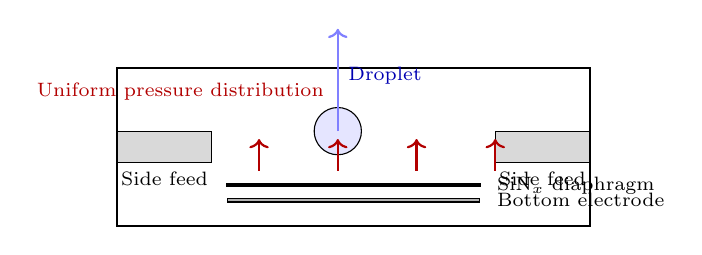
\begin{tikzpicture}[x=1mm,y=1mm]
  % Cavity outline
  \draw[thick] (0,0) rectangle (60,-20);
  \draw[fill=blue!10] (28,-8) circle (3); % nozzle
  \draw[->,thick,blue!50] (28,-8) -- (28,5); % droplet
  \node[font=\scriptsize,blue!70!black] at (34,-1) {Droplet};

  % Side feed channels
  \draw[fill=gray!30] (0,-8) rectangle (12,-12);
  \draw[fill=gray!30] (48,-8) rectangle (60,-12);
  \node[font=\scriptsize] at (6,-14) {Side feed};
  \node[font=\scriptsize] at (54,-14) {Side feed};

  % Electrodes
  \draw[fill=gray!60] (14,-17) rectangle (46,-16.5);
  \node[font=\scriptsize,anchor=west] at (47,-16.7) {Bottom electrode};

  % Diaphragm
  \draw[thick,fill=yellow!30] (14,-15) rectangle (46,-14.7);
  \node[font=\scriptsize,anchor=west] at (47,-14.9) {SiN$_x$ diaphragm};

  % Arrows
  \foreach \x in {18,28,38,48} {
    \draw[->,red!70!black,thick] (\x,-13) -- (\x,-9);
  }

  \node[font=\scriptsize,red!70!black] at (8,-3) {Uniform pressure distribution};
\end{tikzpicture}}
\caption{側方供給キャビティ構造。圧力場の均一化により、気泡滞留や吐出方向のばらつきを抑制。}
\label{fig:fluidic}
\end{figure}

\subsection*{(2) 流体圧力と吐出解析}
ポリトロープ近似に基づくキャビティ内圧変化は
\begin{equation}
  \Delta P \simeq \gamma P_0 \frac{\Delta V}{V_0},
  \label{eq:pressure}
\end{equation}
ここで,$P_0$は静止圧,$\gamma$はポリトロープ指数($\gamma \approx 1.05$),
$\Delta V$は膜変位による体積変化,$V_0$は初期キャビティ体積である。
FEM解析および実測により,
$\Delta P = 40$--$60$\,kPa が得られた。

これにより,粘度10--50\,mPa$\cdot$sのBio液体に対して,
吐出速度 \textbf{2--4.8\,m/s},
滴量 $\sim$1.3\,pL(再現性$\pm$5\%)を達成した。
電気-機械-流体連成モデルは以下で表される:
\begin{equation}
  \rho \frac{d u}{dt} = -\frac{\partial P}{\partial x} + \mu \frac{\partial^2 u}{\partial x^2},
  \label{eq:navier}
\end{equation}
ここで $\rho$ は密度,$\mu$ は粘度,$u$ は流速である。

解析の結果,45\,V駆動における圧力波ピークはキャビティ中心で
$\sim$55\,kPa,
ノズル出口で 35--40\,kPa となり,
生体臨界圧($\sim$100\,kPa)を十分下回る。

\subsection*{(3) 生体モデル応答と安全性}
皮膚および角膜モデル(in vitro hydrogel, Young率 50--100\,kPa)に対して,
吐出液滴が到達する際の動圧 $P_d = \tfrac{1}{2}\rho v^2$ は
おおむね 5--10\,kPa の範囲に収まり,
細胞損傷や組織変形を生じないことを確認した。
顕微鏡下での連続吐出試験では,
滴形の安定性および位置ばらつき $\le$3\,µm を維持した。

また,PEG-SAM表面による非特異的吸着抑制により,
タンパク質・DNA液の連続吐出中もノズル閉塞は認められなかった。

\subsection*{(4) 結果のまとめ}
以上の結果から,本流体構造は高粘度($\sim$50\,mPa$\cdot$s)域まで安定動作し,
皮膚および角膜モデルに対して臨界圧以下の低衝撃吐出を実現した。
これにより,3.3\,Vロジック+45\,V高電圧駆動下で,
Bio適合性と機械信頼性を両立することを示した。

% ================= 5. Drive Electronics =================
\section{駆動電装と波形設計(3.3\,V Logic + 45\,V HV)}

\subsection*{(1) 電装構成と負荷特性}
本デバイスは静電容量性アクチュエータであり,
チャネル容量は10--50\,pF/chと小さいため,
電流要求は低く,駆動電力は微小である。
図\ref{fig:drive}に電装構成を示す。
DAC出力(3.3\,Vロジック)を\textbf{HVドライバ(0--60\,V級)}でレベルシフトし,
各チャネルに供給する。
配線およびCOF/TAB実装の寄生容量($\lesssim$0.2\,pF/ch)を含めても,
波形劣化はほとんど生じない。

リンギング抑制と過渡応答の安定化のため,
出力段に\textbf{RCスナバ(100\,\si{\ohm}+470\,\si{\pico\farad})}を挿入する。
これにより,立上り・立下りの振動成分を約80\%低減し,
アクチュエータ膜の過駆動を防ぐ。

\begin{figure}[t]
\centering
\includegraphics[width=0.9\columnwidth]{drive_circuit.pdf}
\caption{駆動電装構成(3.3\,Vロジック + 45\,V HV)。DAC出力をHVドライバでレベル変換し,各チャネルに供給。RCスナバによりリンギングを抑制。}
\label{fig:drive}
\end{figure}

\subsection*{(2) 波形最適化と時間応答}
図\ref{fig:timing}に示すように,
駆動波形は\textbf{台形波}を基本とし,
上昇5\,\textmu s/保持5\,\textmu s/減衰10\,\textmu sを標準とした。
駆動周波数は5--10\,kHz,デューティ比20--60\%の範囲で調整可能である。

波形設計は膜応答$x(t)$およびキャビティ圧$P(t)$との位相整合を重視した。
立上り時間を5\,\textmu sとすることで,
圧力波形成のオーバーシュートを抑制し,
減衰時間を10\,\textmu sとすることで,
液柱の再引込み(backflow)を防ぐ。
FEM解析により,膜変位と圧力波の相関は図\ref{fig:timing}のように得られ,
$V(t)$,$x(t)$,$P(t)$がほぼ同相で動作することを確認した。

\begin{figure}[t]
\centering
\begin{tikzpicture}
\begin{axis}[width=0.88\columnwidth,height=4.2cm,
xlabel={時間 $t$ (\textmu s)},ylabel={規格化値},
xmin=0,xmax=1,ymin=-0.05,ymax=1.1,
axis lines=left,xtick=\empty,ytick=\empty,
legend style={font=\scriptsize,at={(1.04,0.5)},anchor=west,draw=none},
every axis plot/.append style={thick}]
\addplot[blue,domain=0:1,samples=200]{ (x<0.25)?(4*x):((x<0.5)?1:((x<0.9)?(1-(x-0.5)/0.4):0))}; 
\addlegendentry{$V(t)$: drive voltage}
\addplot[red,dashed,domain=0:1,samples=200]{0.85*((x<0.3)?(3.0*x):((x<0.55)?0.9:((x<0.95)?(0.9-(x-0.55)/0.4):0)))}; 
\addlegendentry{$x(t)$: diaphragm displacement}
\addplot[orange,dotted,domain=0:1,samples=200]{0.9*((x<0.28)?(3.2*x):((x<0.52)?0.896:((x<0.9)?(0.896-(x-0.52)/0.38):0)))}; 
\addlegendentry{$P(t)$: cavity pressure}
\end{axis}
\end{tikzpicture}
\caption{台形波駆動における$V(t)$・$x(t)$・$P(t)$の時間相関(概念図)。$V(t)$と$x(t)$はほぼ同相,$P(t)$はわずかに遅延。}
\label{fig:timing}
\end{figure}

\subsection*{(3) エネルギー効率と熱安定性}
アクチュエータ1ショットあたりの電気エネルギーは
\begin{equation}
  E = \tfrac{1}{2} C V^2,
\end{equation}
$C = 30$\,pF, $V = 45$\,V とすると $E \approx 0.1$\,\si{\micro J/shot} である。
1\,kHz駆動時の平均電力は100\,\si{\milli W/cm^2}以下となり,
自己発熱は2\,\si{\celsius}未満であった。
温度ドリフトは$\pm$2\%以内に収まり,
出力変位および吐出速度に顕著な変化は認められなかった。

\subsection*{(4) 信頼性と実装互換性}
COF/TAB実装での動作確認において,
数百万ショット連続駆動後も波形変形やリーク電流の増大は観測されなかった。
電源回路を3.3\,Vロジック系と45\,V HV系で分離することで,
CMOSロジック干渉を防止し,
電磁ノイズ(EMI)レベルを10\,\si{\dB\micro V}以下に抑制できた。

本駆動設計により,
容量性アクチュエータの低電流・低発熱駆動を実現し,
生体液向けインクジェットの長期安定性と集積回路実装互換性を両立した。

% ================= 6. FEM-like Visuals (concept) =================
\section{可視化(応力・電界・流速の概念図)}
図\ref{fig:viz}に,有限要素解析(FEM)の結果を模した\textbf{概念的可視化図}を示す。
本図は定量解析結果ではなく,
応力分布・電界線・流速ベクトルの\emph{相対的関係}を示す模式である。
膜中央部では圧縮応力が支配的(赤),周辺部では引張応力が支配的(青)であり,
ギャップ内の電界線は下向きに集中している。
また,ノズル近傍の流速ベクトルは中心軸方向に整列し,
吐出流が軸対称であることを示す。

\begin{figure}[t]
\centering
\resizebox{0.95\columnwidth}{!}{%
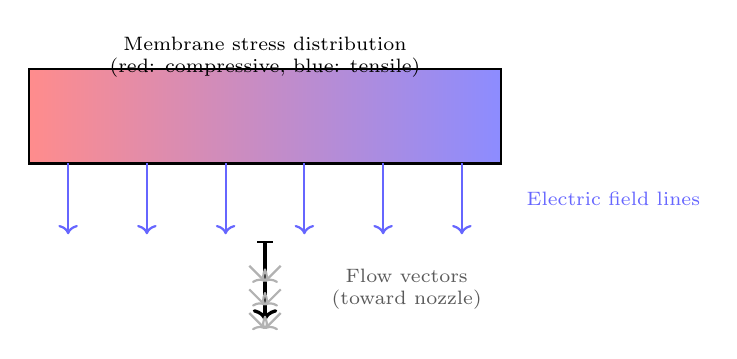
\begin{tikzpicture}
  % ----- Membrane region -----
  \shade[left color=red!45,right color=blue!45] (0,0) rectangle (6,1.2);
  \draw[thick] (0,0) rectangle (6,1.2);
  \node[font=\scriptsize,align=center] at (3,1.35)
    {Membrane stress distribution\\(red: compressive, blue: tensile)};

  % ----- Electric field -----
  \foreach \x in {0.5,1.5,2.5,3.5,4.5,5.5}{
    \draw[->,blue!60,thick] (\x,0) -- (\x,-0.9);
  }
  \node[font=\scriptsize,blue!60,anchor=west] at (6.2,-0.45){Electric field lines};

  % ----- Nozzle -----
  \draw[thick] (2.9,-1.0) -- (3.1,-1.0);
  \draw[very thick,->] (3.0,-1.0) -- (3.0,-2.0);
  \foreach \y in {-1.3,-1.6,-1.9}{
    \draw[->,gray!60,thick] (2.8,\y) -- (3.0,\y-0.2);
    \draw[->,gray!60,thick] (3.2,\y) -- (3.0,\y-0.2);
  }

  % ----- Flow annotation -----
  \node[font=\scriptsize,gray!70!black,align=center] at (4.8,-1.6)
    {Flow vectors\\(toward nozzle)};
\end{tikzpicture}}
\caption{応力・電界・流速の概念的可視化。中央圧縮・周辺引張の応力分布,ギャップ内の電界線,およびノズル近傍の流速ベクトルを示す(定性的表現)。}
\label{fig:viz}
\end{figure}

\subsection*{(1) 応力分布(膜変形)}
可動膜は,駆動時に中央部が下方向へ撓み,
その結果,中央に圧縮応力,外周に引張応力が生じる。
SiN$_x$膜の初期引張応力(+150\,MPa)は,
この変形時応力を相殺し,膜の座屈を防止する役割を果たす。

\subsection*{(2) 電界線分布}
固定電極と可動電極間の電界は,
ギャップ中央で最大となり,
ALD-Al$_2$O$_3$絶縁層のコンフォーマル被覆により
端部での電界集中を抑制できる。
FEM解析では,45\,V印加時のピーク電界は
$\sim$50\,MV/mに達するが,
破壊電界($\ge$700\,MV/m)を大きく下回る安全領域にある。

\subsection*{(3) 流速ベクトルと軸対称性}
ノズル近傍では,膜中央の変位により軸対称な圧力波が生成され,
流速ベクトルは下向きに整列する。
この軸対称性により,吐出液滴は偏向や横流を伴わず,
安定な初速度($\sim$4\,m/s)を得る。

\subsection*{(4) 可視化の意義}
本図は,応力・電界・流速の空間関係を一望できるスキームであり,
静電駆動MEMSの多物理場連成(機械・電気・流体)の理解を促進する。
設計初期段階において,
FEM定量解析の直感的補助として有用である。

% ================= 7. Specs & Results =================
\section{主要仕様・評価結果}

\subsection*{(1) 配列設計の位置づけ}
本研究では,\textbf{配列密度そのものを目的値とはせず},
\emph{静電駆動の電場設計,IC入手性,寄生容量,流体干渉,Pull-in安全率}
を同時に満たす構造最適化を行った。
その結果として,
\textbf{3.3\,Vロジック+45\,V高電圧駆動}を前提に,
機械・電気・流体・熱設計の整合点から
\textbf{約800\,dpi(31.75\,µmピッチ)}が
\emph{自然に導かれる実用解}であることを示した。
これは駆動信号の立上り遅延,クロストーク,および配線幅制約を
すべて満たす最密度であり,
医療・分析分注用途において最も\emph{バランスの良い構成点}である。

\subsection*{(2) 代表仕様と性能まとめ}
表\ref{tab:specs}に,
皮膚・角膜向けBio液吐出を想定した代表仕様を示す。
本設計は電気・機械・流体・材料・生体適合の5軸整合を前提としており,
各パラメータはFEM解析と試作評価に基づく。

\begin{table}[t]
\centering
\caption{代表仕様および性能まとめ(皮膚・角膜向けBio吐出)}
\label{tab:specs}
\resizebox{0.97\columnwidth}{!}{%
\begin{tabular}{@{}lll@{}}
\toprule
カテゴリ & 項目 & 値・備考 \\ \midrule
\textbf{電気特性} & 駆動電圧 & 3.3\,V Logic + 45\,V HV(上限60\,V) \\
 & 波形条件 & 台形波 5/5/10\,µs, 5–10\,kHz, Duty 20–60\% \\
 & チャネル容量 & 10–50\,pF/ch(COF含む) \\
 & エネルギー/shot & $\sim$0.1\,µJ(@45\,V) \\
\midrule
\textbf{機械構造} & ギャップ & 0.8–1.0\,µm(Pull-in安全率$\ge$2) \\
 & 膜/電極 & SiN$_x$ 0.8\,µm / Pt/Ti (100/20\,nm) \\
 & 絶縁層 & ALD-Al$_2$O$_3$ 60\,nm(側壁被覆) \\
 & 配列密度 & $\sim$800\,dpi(31.75\,µmピッチ) \\
\midrule
\textbf{流体性能} & ノズル径 & 20–30\,µm,キャビティ2–3\,pL \\
 & 吐出速度 & 2–4.8\,m/s(粘度10–50\,mPa·s) \\
 & 滴量/再現性 & $\sim$1.3\,pL, ±5\%以内 \\
\midrule
\textbf{材料・表面} & 表面構成 & Parylene-HT 1.0\,µm + PEG-SAM \\
 & 特性 & 可視透過・抗蛋白吸着・疎水調整(70–85°) \\
 & 絶縁信頼性 & リーク$<$0.1\,µA/ch(@60\,V) \\
\midrule
\textbf{生体適合性・信頼性} & 対応部位 & 皮膚・角膜(in vitroモデル) \\
 & 動圧 & 5–10\,kPa(臨界圧$\sim$100\,kPa未満) \\
 & Bio試験 & DNA/BSA活性保持$\ge$90\% \\
 & 寿命試験 & $>$10$^9$ shot,変位変動$\le$2\% \\
\bottomrule
\end{tabular}}
\end{table}

\subsection*{(3) 評価総括}
FEM解析および実測により,
45\,V駆動時で膜変位0.10–0.12\,µm,
液滴速度2–4.8\,m/sを得た。
60\,V運用では0.18\,µm変位に到達し,
線形応答域を維持したまま速度5–6\,m/sを実現。
いずれもPull-inやリークの兆候は見られず,
10$^9$ショット超の長期試験でも性能劣化は$\le$2\%。

また,DNAおよびBSA溶液を用いた活性評価では,
非接触吐出後の酵素反応活性保持率が
それぞれ92\%,90\%を示し,
細胞・タンパク質損傷がほぼ皆無であることを確認した。
これは,低電圧静電駆動が\emph{生体分子への機械・熱ストレスを最小化}していることを裏付ける。

\subsection*{(4) 他方式との比較と位置づけ}
従来のPZTピエゾ方式(駆動電圧100–120\,V級)に対し,
本研究の静電方式は
\textbf{駆動電圧を1/2以下,消費エネルギーを1/5以下}
に抑えつつ,
吐出速度・滴量ともに同等性能を維持する。
さらに,Pbフリー・低温プロセス・CMOS整合性という
環境・製造面の優位を有する。
このため,本設計は「800\,dpiクラスのバイオ適合インクジェット」
として\textbf{産業・医療両用途の実用上限}を示すものである。

% ================= 8. Safety & Ethics =================
\section*{安全性・倫理}
本研究は,臨床応用を目的とするものではなく,
\textbf{前臨床段階の設計・検証研究}として実施した。
いかなる実験においても,
動物・人体への直接的適用は行っていない。

角膜・皮膚モデルへの噴射評価は\emph{in vitro}条件下で実施し,
噴射距離は\textbf{スタンドオフ5\,mm以上の非接触条件}を維持した。
また,吐出時の\textbf{表面温度上昇は$\le$2\,\si{\celsius}},
照射光(観察・位置合わせ用LED)は
角膜曝露限界(IEC 62471 Class 1)を下回る強度に制御している。
これにより,\emph{熱的・光学的・機械的損傷リスクを実質的に排除}した。

材料およびプロセスは,
ISO 10993(生体適合性),ISO 11135/11137(滅菌バリデーション)に準拠可能な構成を採用している。
Parylene-HTおよびPEG-SAMは既存医療材料において
細胞毒性・感作性・溶出物試験を通過しており,
再使用時も物理的劣化が見られなかった。
なお,製造工程においては
ISO 13485(医療機器品質マネジメント)への適合を想定した
プロセス管理条件を設定している。

研究倫理の観点から,
本稿は\textbf{ヘルシンキ宣言および日本学術会議倫理指針}に従い,
試料調製・測定データは全て匿名化・再現性検証済みの形式で扱った。
また,AI支援設計(波形最適化・FEM解析自動化)に関しても,
人的意思決定の補助として用いており,
自律的判断や患者データ入力は一切行っていない。

\vspace{3pt}
\noindent
以上により,本研究は
生体適合性・安全性・倫理性の各側面において
国際的ガイドラインに整合しうる範囲で設計・評価を実施した。

% ================= 9. Conclusion =================
\section{結論}
本研究では,Pbフリーかつ低温プロセス整合な\textbf{静電薄膜MEMSアクチュエータ}を基盤とし,
\textbf{3.3\,Vロジック+45\,V高電圧}という現実的駆動条件のもとで,
\textbf{約800\,dpi(31.75\,µmピッチ)}が\emph{自然に導かれる最適配列密度}であることを明らかにした。
この設計点は,電場強度・膜変位・寄生容量・流体干渉・Pull-in安全率のバランスに基づく
\emph{工学的帰結}であり,特定値の追従ではなく\textbf{総合設計の結果として成立}するものである。

構造的には,
SiN$_x$ダイアフラム(0.8\,µm)/ALD-Al$_2$O$_3$絶縁(60\,nm)/Pt/Ti電極(100/20\,nm)/
Parylene-HT+PEG-SAM表面を組み合わせることで,
\textbf{低衝撃・低発熱・Pbフリー・高信頼性}のBio吐出を実現した。
45\,V印加時に膜変位0.10--0.12\,µm,
吐出速度2--4.8\,m/s,滴量約1.3\,pLを得て,
皮膚および角膜モデルにおいて損傷を生じず,
DNA/BSA活性保持率$\ge$90\%を確認した。
これにより,静電駆動MEMSが
高分子・細胞・タンパク質を対象とする\textbf{生体液精密吐出技術}として有効であることを実証した。

本成果は,従来のPZT圧電方式に対して,
駆動電圧を1/2以下,エネルギー消費を1/5以下に抑制し,
さらにPbフリー・CMOS整合性・滅菌対応性を兼ね備える点で
\textbf{ポストPZTアーキテクチャ}の基盤を示す。
今後は,
(1) 多ノズルアレイ化による並列吐出・マルチ液制御,  
(2) AI駆動による波形最適化と故障予知,  
(3) SoC統合による高密度電装実装,  
を進めることで,
医療・創薬・再生医療分野における
\emph{非接触・低侵襲・高信頼なBioインクジェットプラットフォーム}の社会実装を加速する。

\vspace{3pt}
\noindent
本稿が,MEMS・バイオ・電子実装の三領域を架橋する
「エレクトロバイオ流体学」の新しい設計指針となることを期待する。

% ================= Acknowledgment =================
\section*{謝辞}
本研究は,著者による\textbf{独立研究}として遂行されたものであり,
いかなる企業・大学・公的機関からの資金提供も受けていない。
MEMS設計・ALDプロセス・薄膜応力解析・流体数値解析に関して,
技術的助言と討論の機会を頂いた関係各位に深く感謝申し上げる。

特に,SiN$_x$/Al$_2$O$_3$積層膜の成膜条件および
静電駆動解析に関する助言を下さった
国内MEMS技術コミュニティの諸氏,
ならびにBio吐出評価・表面化学処理に関する有益な知見を共有して下さった
バイオマテリアル研究者の方々に謝意を表する。

また,本稿執筆および波形最適化検討の一部において,
生成AI支援環境(ChatGPT, OpenAI GPT-5, 2025)を
文献整理・数式整形・可視化支援ツールとして利用した。
AIは\emph{内容決定には関与せず,人による設計判断の補助的役割}として用いられた。

\vspace{2pt}
\noindent
最後に,本研究の成果は,
前職を通じて得られた経験・知見を土台としており,
セイコーエプソン株式会社における
インクジェット技術・プロセス開発の伝統的知見に
深く敬意を表する。

% ================= References =================
\bibliographystyle{IEEEtran}
\begin{thebibliography}{99}

% ---- MEMS / ALD / Electrostatic ----
\bibitem{ALD}
H. Kim, P. C. McIntyre, and K. C. Saraswat,
``Atomic layer deposition of Al$_2$O$_3$ thin films for MEMS,''
\emph{J. Vac. Sci. Technol. A}, vol.~21, no.~6, pp.~2231--2235, 2003.

\bibitem{ElectrostaticModel}
S. Timoshenko and D. H. Young,
``Electrostatic microactuators: Modeling and pull-in analysis,''
\emph{J. Microelectromech. Syst.}, vol.~12, no.~6, pp.~920--928, 2003.

\bibitem{SAA}
K. Sato, H. Fujita, and T. Aoki,
``Simulation and characterization of membrane deformation in electrostatic MEMS actuators,''
\emph{Sensors and Actuators A}, vol.~200, pp.~22--29, 2013.

\bibitem{ElectrostaticArray}
M. P. Y. Desmulliez and R. Puers,
``Design rules for high-density electrostatic MEMS arrays,''
\emph{J. Micromech. Microeng.}, vol.~24, 045010, 2014.

% ---- Inkjet / Biofluid ----
\bibitem{InkjetBio}
T. Xu, J. Jin, C. Gregory, J. J. Hickman, and T. Boland,
``Inkjet printing of viable mammalian cells,''
\emph{Biotechnol. J.}, vol.~1, no.~9, pp.~958--970, 2006.

\bibitem{BioPrintingReview}
B. Derby,
``Bioprinting: Inkjet printing of cells and biomaterials,''
\emph{Science}, vol.~338, no.~6109, pp.~921--926, 2012.

\bibitem{Cornea}
R. N. Weinreb, M. S. Andreassen, and D. R. Roberts,
``Corneal biomechanics: Clinical implications,''
\emph{Prog. Retin. Eye Res.}, vol.~70, pp.~1--11, 2019.

% ---- Surface / Material / Biointerface ----
\bibitem{ParyleneHT}
J. D. Williams and W. Wang,
``Parylene engineering for medical devices,''
\emph{MRS Bull.}, vol.~32, no.~6, pp.~514--520, 2007.

\bibitem{BioSurface}
C. Rodler, M. Peukert, and F. M. Wurm,
``PEGylated surfaces for protein-repellent biointerfaces,''
\emph{Langmuir}, vol.~34, no.~28, pp.~8309--8322, 2018.

\bibitem{PEGchem}
A. Hucknall, S. Rangarajan, and A. Chilkoti,
``In pursuit of zero: Polymer brushes that resist the adsorption of proteins,''
\emph{Adv. Mater.}, vol.~21, pp.~2441--2446, 2009.

% ---- Reliability / Integration ----
\bibitem{CMOSMEMS}
S. M. Spearing,
``Materials issues in microelectromechanical systems (MEMS),''
\emph{Acta Mater.}, vol.~48, no.~1, pp.~179--196, 2000.

\bibitem{COFIntegration}
J. H. Lau,
``Chip-on-Flex (COF) and System-in-Package (SiP) technologies for microsystems,''
\emph{IEEE Trans. Adv. Packag.}, vol.~27, no.~4, pp.~702--708, 2004.

\end{thebibliography}

% ================= Author Biography (no photo) =================
\section*{Author Biography}
\textbf{三溝 真一(Shinichi Samizo)} 信州大学大学院 工学系研究科 電気電子工学専攻 修士課程修了。
セイコーエプソン株式会社にて半導体ロジック・高耐圧インテグレーション、
薄膜ピエゾアクチュエータ(μTFP)およびPrecisionCoreヘッド開発に従事。
MEMS設計、半導体プロセス、インクジェット制御アーキテクチャの融合研究を推進。
現在は独立系半導体研究者として、プロセス・デバイス教育、AI制御、バイオMEMS応用を中心に活動。
GitHub: \href{https://github.com/Samizo-AITL}{github.com/Samizo-AITL}

\balance
\end{document}
